\section{Performance Enhancement}



\begin{frame}{A Novel Pre-Processing Method Against Covariate Shift}
    \begin{enumerate}
        \item \textbf{No Prior Shift Knowledge Needed}
        \begin{itemize}
            \item Simplifies implementation by eliminating the need for shift estimation.
            \item Adaptable to various datasets without additional shift information.
        \end{itemize}
        
        \item \textbf{Built-in Regularization}
        \begin{itemize}
            \item Prevents overfitting by introducing controlled noise.
            \item Enhances model generalization on unseen data.
        \end{itemize}
    \end{enumerate}
\end{frame}



\begin{frame}{The R.A.W. Method}
    \begin{columns}[T]
        
        \begin{column}{0.35\textwidth}
            \begin{block}{R.A.W.}
                \begin{itemize}\LARGE
                    \item \textbf{R}andom
                    \item \textbf{A}ugmentation
                    \item \textbf{W}alk
                \end{itemize}
            \end{block}
        \end{column}
        
        \vline\hspace{1em} 
        
        % Second Column: Algorithm
        \begin{column}{0.60\textwidth}
            \begin{algorithm}[H]
                \setstretch{1.2}
                \caption{R.A.W. Pre-Processing Algorithm}
                \begin{algorithmic}[1]
                    \State \textbf{Input:} $Data_{\text{train}}$, $Size$, $N$, $\varepsilon$.
                    
                    \State $Data_{\%} \gets$ random subset of $N\%$ of $Data_{\text{train}}$
                    
                    \For{each $x_i$ in $Data_{\%}$}
                        \State $x_i' \gets$
                        \Statex \quad 
                        $\begin{cases}
                            x_i + \varepsilon & \text{with probability } 0.5 \\
                            x_i - \varepsilon & \text{with probability } 0.5
                        \end{cases}$
                        \State $y_i' \gets y_i$
                    \EndFor
                    
                    \State $Data_{\text{aug}} \gets Data_{\text{new}} \cup Data_{\%}$
                    
                    \State $Data_{\text{final}} \gets \text{Downsample}(Data_{\text{aug}}, Size)$
                    
                    \State \textbf{Return} $Data_{\text{final}}$
                \end{algorithmic}
            \end{algorithm}
        \end{column}
    \end{columns}
\end{frame}


\begin{frame}{Classify With Gradient Boosting Using R.A.W.}
    \begin{itemize}
        \item **Step 1:** Apply the R.A.W. pre-processing method to the training data to address covariate shift.
        \item **Step 2:** Train a Gradient Boosting Classifier on the augmented dataset.
        \item **Step 3:** Evaluate the model's performance on shifted test sets.
    \end{itemize}
    
    \vspace{1em}
    \begin{figure}
        \centering
        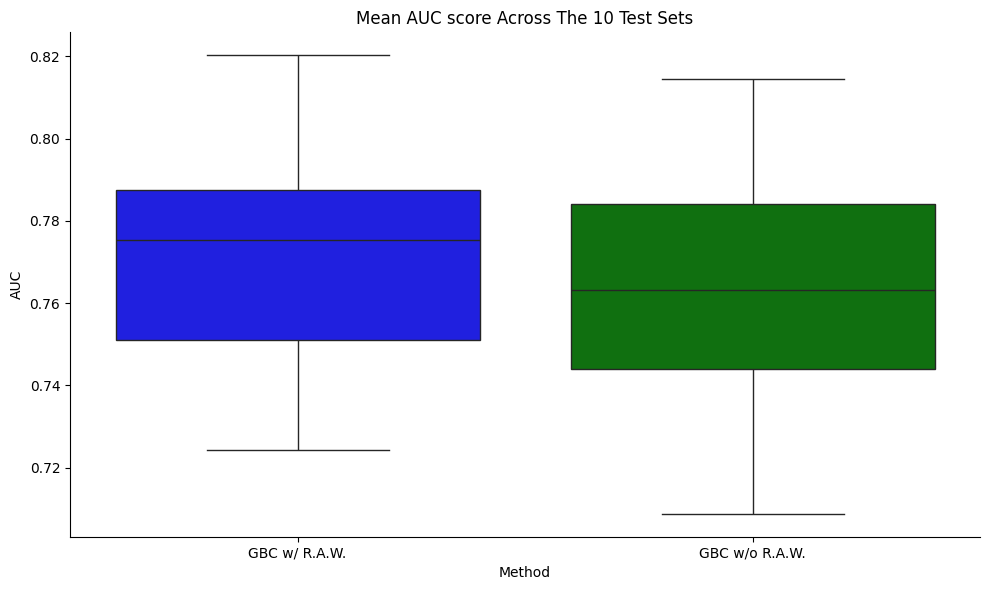
\includegraphics[width=0.45\textwidth]{MeanAUCscoreacross10.png}
        \hfill
        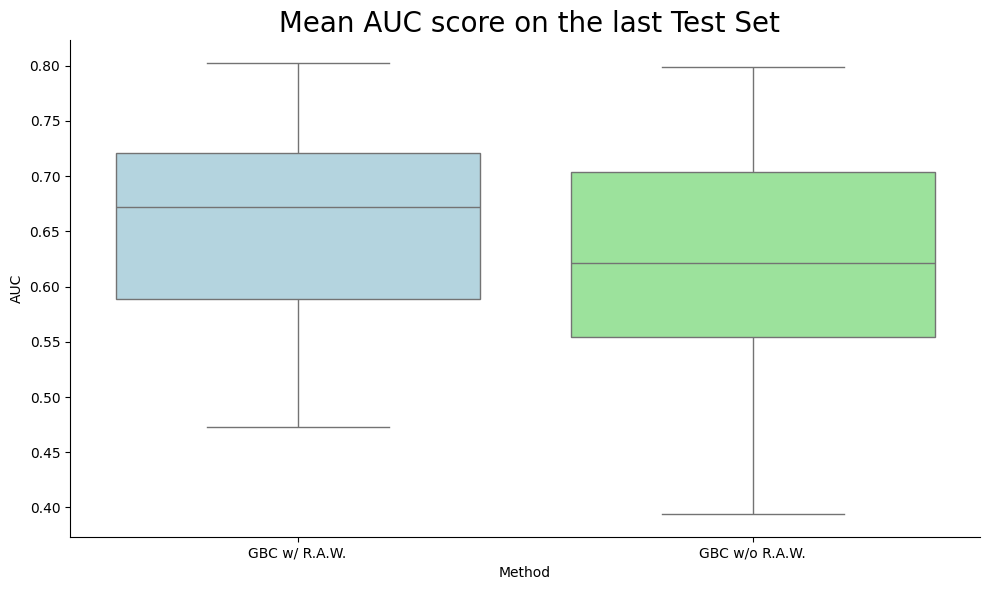
\includegraphics[width=0.45\textwidth]{MeanAUCscoreLAST.png}
    \end{figure}
    
\end{frame}



\begin{frame}{A Statistical Analysis Of The Results}
    \begin{itemize}
        \item \textbf{Null Hypothesis ($H_0$):} $\Delta\bar{\mu} = \overline{\text{AUC}}_{\text{R.A.W.}} - \overline{\text{AUC}}_{\text{base}} = 0$ \\
        \quad The R.A.W. method does not improve the AUC score of the Gradient Boosting Classifier.
        
        \item \textbf{Alternative Hypothesis ($H_1$):} $\Delta\bar{\mu} = \overline{\text{AUC}}_{\text{R.A.W.}} - \overline{\text{AUC}}_{\text{base}} \neq 0$ \\
        \quad The R.A.W. method improves the AUC score of the Gradient Boosting Classifier.
        
        \item \textbf{Test Used:} Paired t-test on 50 independent $\overline{\text{AUC}}$ differences.
    \end{itemize}
    
    \vspace{1em}
    
    \begin{table}[h!]
        \centering
        \small
        \begin{tabular}{lcccc}
            \toprule
            & $\Delta\bar{\mu}$ & t-stat & p-value & 95\% CI \\
            \midrule
            $\Delta\overline{\text{AUC}}$* & 0.0083 & 8.75  & $1.39 \times 10^{-11}$ & [0.006, 0.010] \\
            $\Delta\overline{\text{AUC}}_{\text{last}}$** & 0.0235 & 10.59 & $2.86 \times 10^{-14}$ & [0.019, 0.028] \\
            \bottomrule
        \end{tabular}
        \caption{Statistical Test Results}
        \label{tab:stat_results}
    \end{table}
    
    \vspace{0.5em}
    
    \begin{footnotesize}
        * Mean AUC score difference across all 10 shifted test sets. \\
        ** Mean AUC score difference on the most shifted test set.
    \end{footnotesize}
   
\end{frame}


\begin{frame}
    \begin{figure}
        \centering
        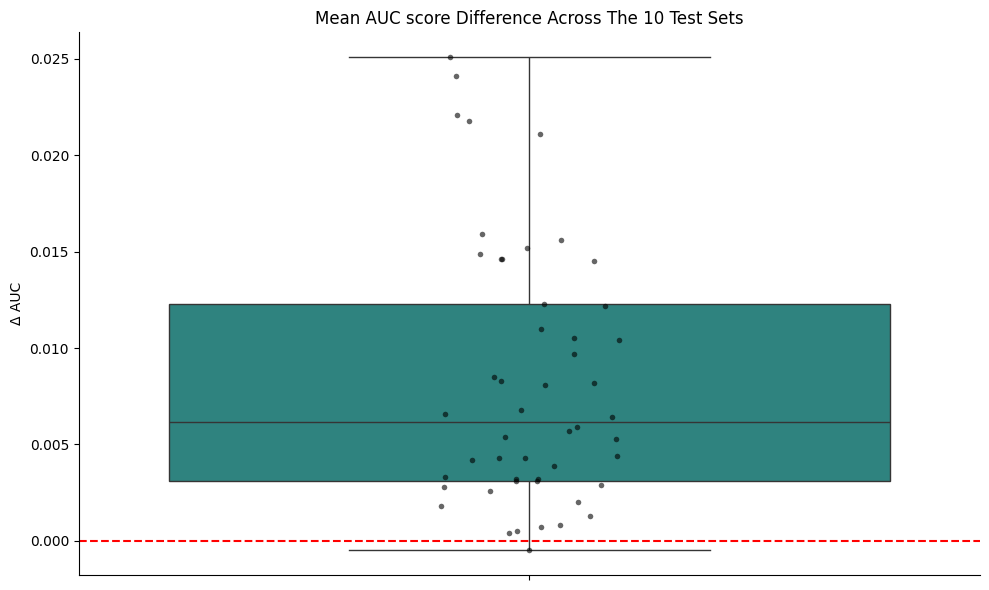
\includegraphics[width=0.45\textwidth]{diffacross10.png}
        \hfill
        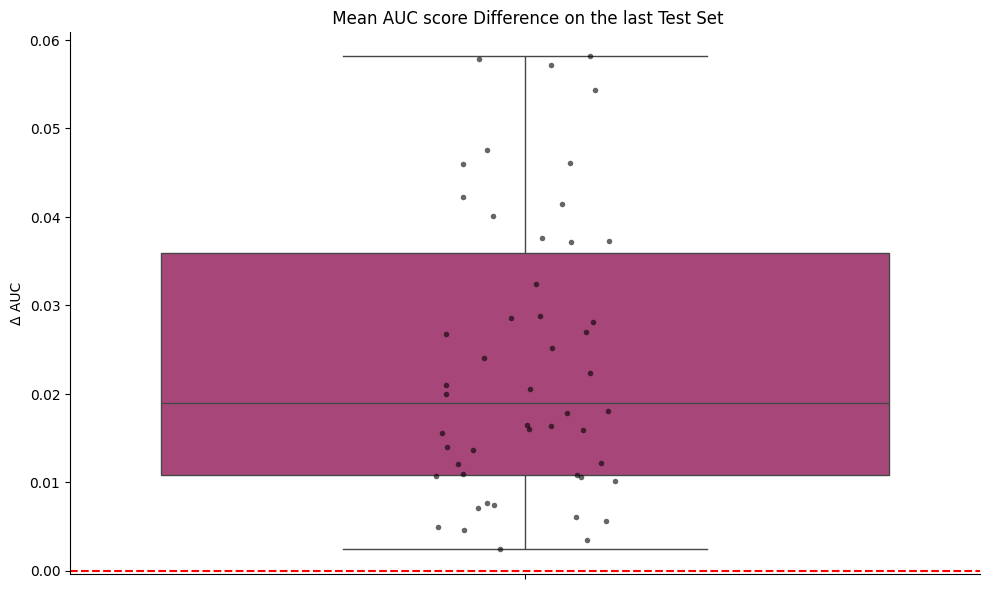
\includegraphics[width=0.45\textwidth]{meandiffLAST.png}
    \end{figure}
\end{frame}

